\subsection{Электронная кодовая книга}
\selectlanguage{russian}

\begin{figure}[bt]
	\centering
	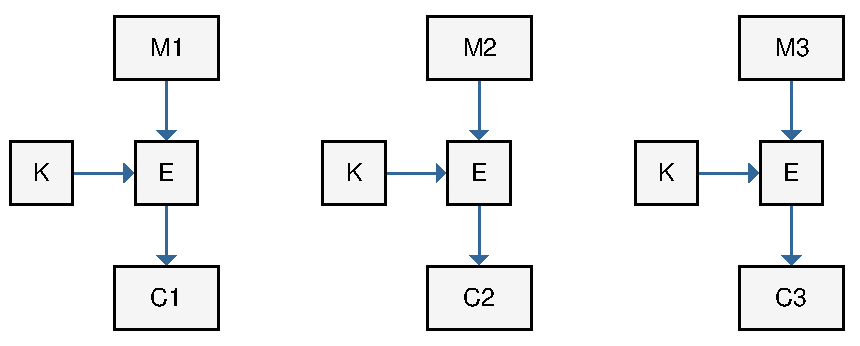
\includegraphics[width=1\textwidth]{pic/ECB}
	\caption{Режим электронной кодовой книги}
	\label{fig:ECB}
\end{figure}

В стандарте ГОСТ 28147-89 данный режим называется \emph{режимом простой замены}.~\cite{GOST-89}

В режиме электронной кодовой книги (\langen{Electronic Code Book, ECB}, рис.~\ref{fig:ECB}) открытый текст в пакете разделён на блоки
    \[ \left[ M_1, M_2, \dots, M_{n-1}, M_n \right]. \]

В процессе шифрования каждому блоку $M_j$ ставится в соответствие шифртекст $C_j$, определяемый с помощью ключа $K$:
    \[ C_j = E_K(M_j), ~ j = 1, 2, \dots, n. \]

Если в открытом тексте есть одинаковые блоки, то в шифрованном тексте им также соответствуют одинаковые блоки. Это даёт дополнительную информацию для криптоаналитика, что является недостатком этого режима. Другой недостаток состоит в том, что криптоаналитик может подслушивать, перехватывать, переставлять, воспроизводить ранее записанные блоки, нарушая конфиденциальность\index{конфиденциальность} и целостность\index{целостность} информации. Поэтому при работе в режиме электронной кодовой книги нужно вводить аутентификацию сообщений.

Шифрование в режиме электронной кодовой книги не использует сцепление блоков и синхропосылку\index{синхропосылка} (вектор инициализации)\index{вектор инициализации}. Поэтому для данного режима применима атака на различение сообщений, так как два одинаковых блока или два одинаковых открытых текста шифруются идентично.

На рис.~\ref{fig:ecb-demo} приведён пример шифрования графического файла морской звезды в формате BMP, 24 бита цветности на пиксель (рис.~\ref{fig:starfish}), блочным шифром AES с длиной ключа 128 бит в режиме электронной кодовой книги (рис.~\ref{fig:starfish-aes-128-ecb}). В начале зашифрованного файла был восстановлен стандартный заголовок формата BMP. Как видно, в зашифрованном файле изображение всё равно различимо.
\begin{figure}[!ht]
    \centering
    \subcaptionbox{Исходный рисунок\label{fig:starfish}}{ 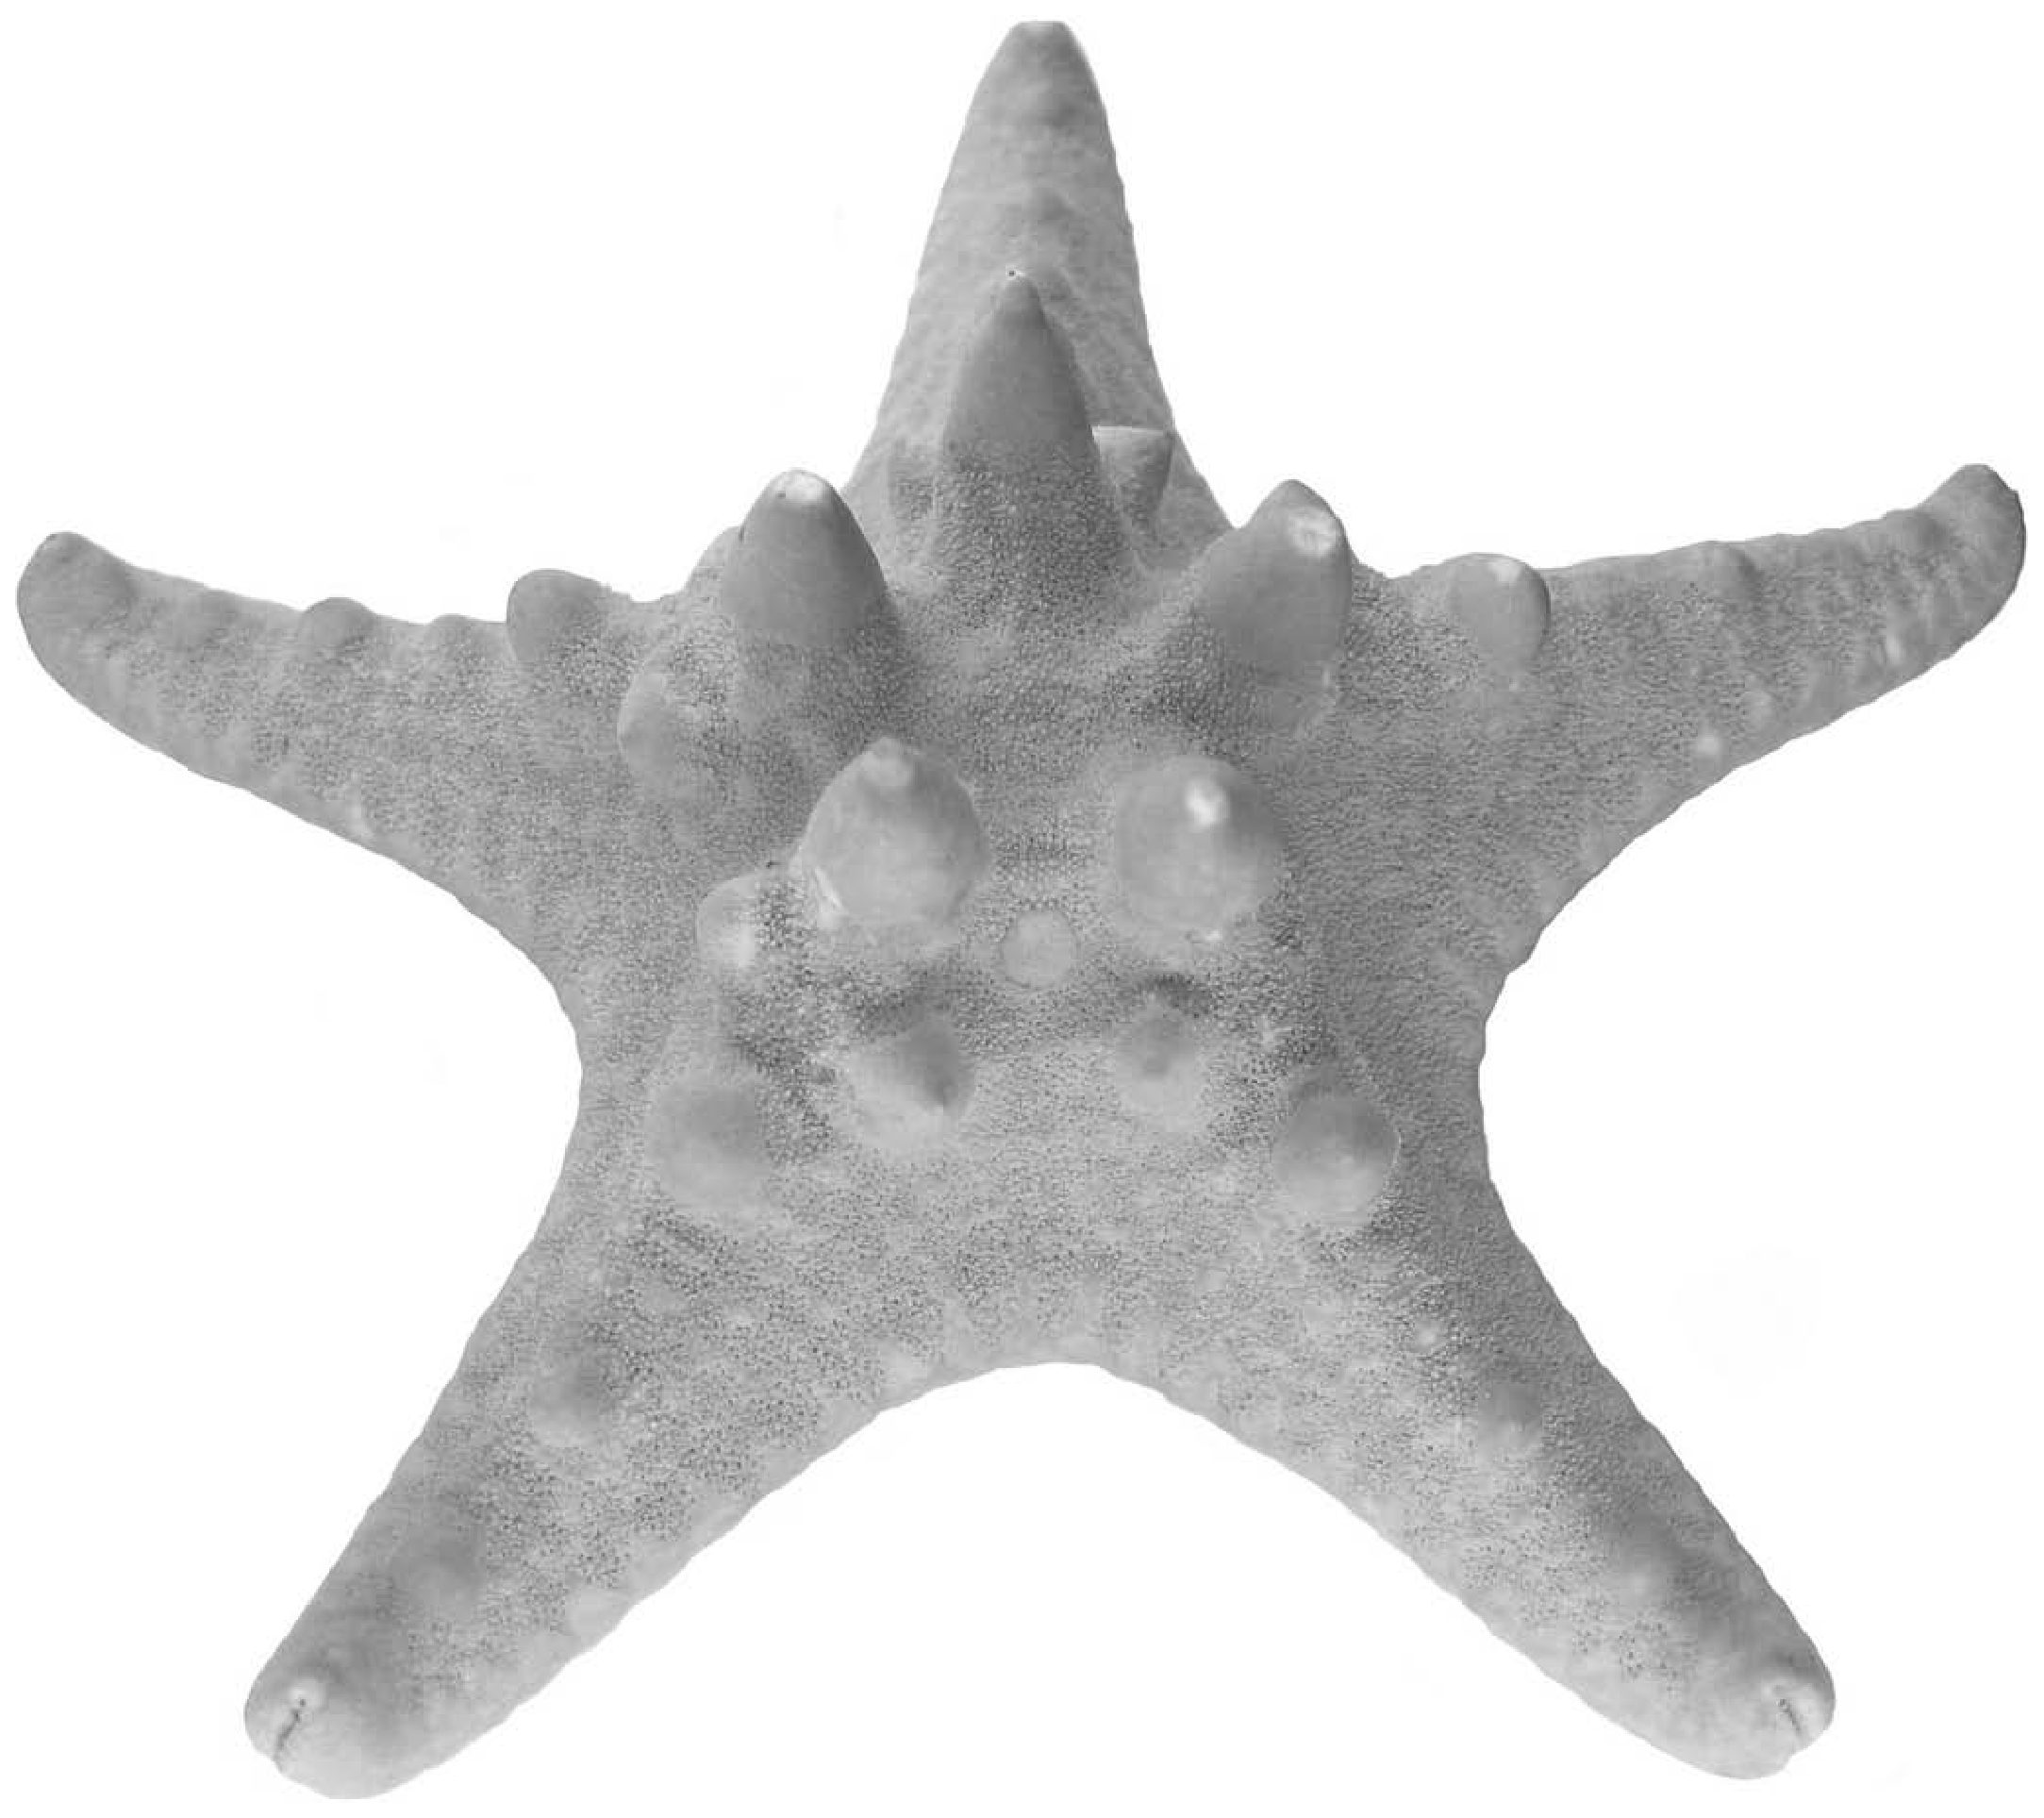
\includegraphics[width=0.45\textwidth]{pic/starfish}}
    ~~~
    \subcaptionbox{Рисунок, зашифрованный AES-128\label{fig:starfish-aes-128-ecb}}{ 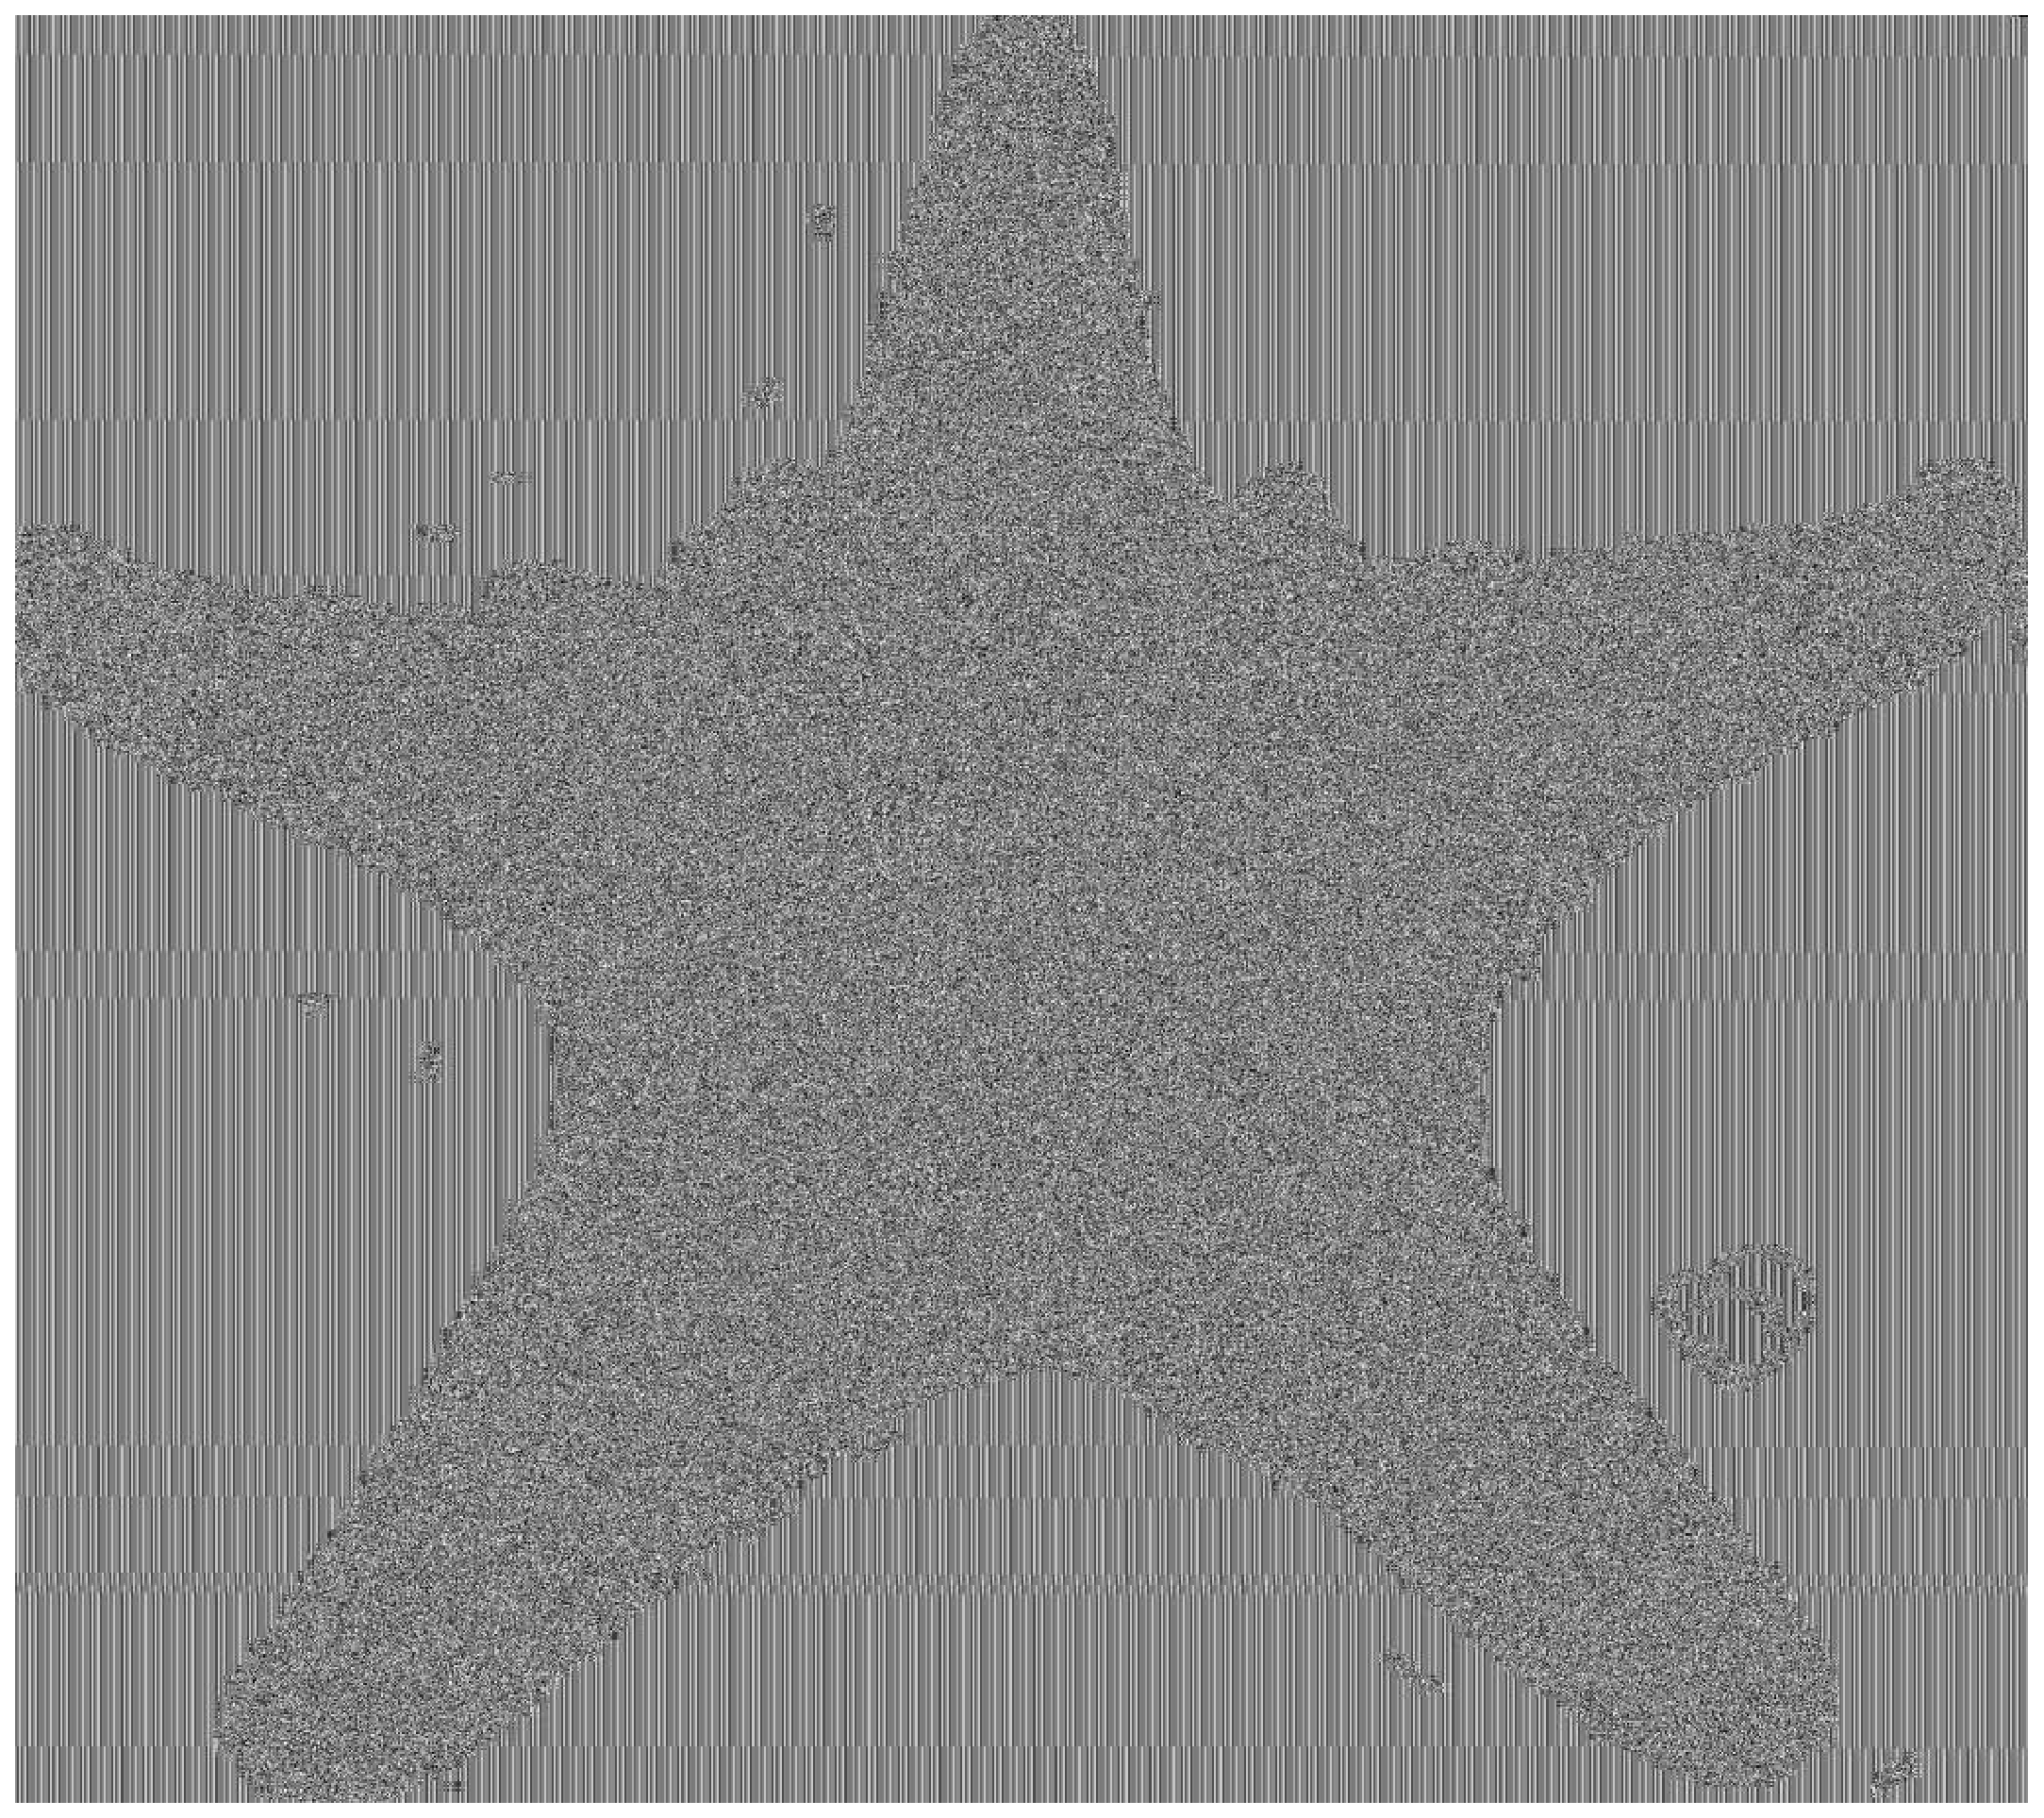
\includegraphics[width=0.45\textwidth]{pic/starfish-aes-128-ecb}}
    \caption{Шифрование в режиме электронной кодовой книги\label{fig:ecb-demo}}
\end{figure}
BMP файл в данном случае содержит в самом начале стандартный заголовок (ширина, высота, количество цветов), и далее идёт массив 24-битовых значений цвета пикселей, взятых построчно сверху вниз. В массиве много последовательностей нулевых байтов, так как пиксели белого фона кодируются 3 нулевыми байтами. В AES размер блока равен 16 байтам, и, значит, каждые $\frac{16}{3}$ подряд идущих пикселей белого фона шифруются одинаково, позволяя различить изображение в зашифрованном файле.

%На рис.~\ref{fig:ecb-demo} приведён пример шифрования графического файла логотипа Википедии в формате BMP, 24 бита цветности на пиксель (рис.~\ref{fig:wikilogo}), блочным шифром AES с длиной ключа 128 бит в режиме электронной кодовой книги (рис.~\ref{fig:wikilogo-aes-128-ecb}). В начале зашифрованного файла был восстановлен стандартный заголовок BMP формата. Как видно, на зашифрованном рисунке возможно даже прочитать надпись.
%\begin{figure}[!ht]
%    \centering
%    \subfloat[Исходный рисунок]{\label{fig:wikilogo}\includegraphics[width=0.45\textwidth]{pic/wikilogo}}
%    ~~~
%    \subfloat[Рисунок, зашифрованный AES-128]{\label{fig:wikilogo-aes-128-ecb}\includegraphics[width=0.45\textwidth]{pic/wikilogo-aes-128-ecb}}
%    \caption{Шифрование в режиме электронной кодовой книги.}
%    \label{fig:ecb-demo}
%\end{figure}

%Возможно воссоздание структуры информации -- например, пингвин на рис.~\ref{fig:tux-ecbmode}. Картинка с пингвином записана в формате BMP и зашифрована DES в режиме электронной кодовой книги.
%\begin{figure}[!ht]
%    \centering
%    \includegraphics[width=0.3\textwidth]{pic/tux-ecb}
%    \caption{Картинка с пингвином, зашифрованная в режиме электронной кодовой книги.}
%    \label{fig:tux-ecbmode}
%\end{figure}

Преимущества:
\begin{itemize}
	\item самый простой в реализации режим работы шифра (<<наивный>>);
	\item возможность параллельного шифрования любого количества блоков открытого текста.
\end{itemize}

Недостатки:
\begin{itemize}
	\item необходимость дополнения открытого текста до размера, кратного размеру блоку шифрования;
	\item сохранение статистических особенностей открытого текста на уровне блоков шифртекста;
	\item ошибка передачи одного бита приводит к ошибке расшифровки целого блока открытого текста;
	\item не обеспечивает целостность.
\end{itemize}

Основным минусом режима является сохранение статистических особенностей открытого текста на уровне шифртекста (одинаковые блоки шифруются одинаково). Причём это поведение сохраняется и между сессиями, что позволяет злоумышленнику, используя информацию из сторонних каналов (например, зная о предпринятых действиях получателя сообщения), составить словарь между переданными блоками шифртекста и предполагаемыми -- открытого текста. То есть злоумышленник может попытаться восстановить соответствующую \emph{кодовую книгу} для данного ключа шифрования и потом восстанавливать сообщения по этой книге без знания ключа шифрования\index{ключ!шифрования}.

Когда говорят про восстановление после ошибок передачи, то рассматривают ситуацию, в которой один или несколько бит одного блока шифртекста поменяли\footnote{В отдельных продвинутых режимах работы блочных шифров рассматривают также варианты потери бит или вставки новых ошибочных, что приводит к изменению размеров переданных блоков и требует дополнительной работы по синхронизации} своё значение в процессе передачи по каналу связи между отправителем (тем, кто шифрует) и получателем (тем, кто расшифровывает). В режиме ECB изменение даже одного бита переданного блока шифртекста приведёт к тому, что весь блок открытого текста будет расшифрован неверно.\footnote{См.~\autoref{section:avalanche_effect}} То есть вместо блока открытого текста получится 64 или 128 бит мусора (случайных бит). Однако все последующие блоки шифртекста, если они будут переданы без ошибок, будут корректно расшифрованы, так как ошибки при передаче одного блока в режиме ECB не влияют на остальные блоки. В других режимах это поведение может отличаться.

Данный режим (как и большая часть остальных рассмотренных режимов) обеспечивает только конфиденциальность\index{конфиденциальность} передачи данных, но не целостность\index{целостность}. В модели активного злоумышленника, если он предполагает о содержимом блоков открытого текста для части шифртекста, он может, например, манипулировать передаваемыми блоками, вставляя, удаляя или меняя блоки местами. Это приведёт к соответствующим изменениям в открытом тексте (и не приведёт к <<мусору>> после расшифровки). Такие изменения могут не быть замечены получателем и привести к таким действиям, которые ожидает злоумышленник, а не легальный отправитель.
